
% Copyright (c) 2015 - 2020 Mario Mlačak, mmlacak@gmail.com
% Licensed and published as Public Domain work.

% One chapter =========================================================
\chapter*{One}
\addcontentsline{toc}{chapter}{One}

\begin{flushright}
\parbox{0.8\textwidth}{
\emph{God is not external to anyone, but is present with all things, though
they are ignorant that he is so. \\
\hspace*{\fill}{\textperiodcentered \textperiodcentered \textperiodcentered \hspace*{0.2em} Plotinus} } }
\end{flushright}

\noindent
One is chess variant which is played on 26 x 26 board, with white and
darker violet fields, and with light purple and fuchsia pieces. Star
colors are reversed colors of ordinary pieces, i.e. fuchsia and light
purple. In algebraic notation, columns are enumerated from 'a' to 'z',
and rows are enumerated from '1' to '26'. A new piece is introduced,
Starchild.

\clearpage % ..........................................................
% Starchild ***********************************************************

\section*{Starchild}
\addcontentsline{toc}{section}{Starchild}

\noindent
\begin{wrapfigure}[11]{l}{0.4\textwidth}
\centering
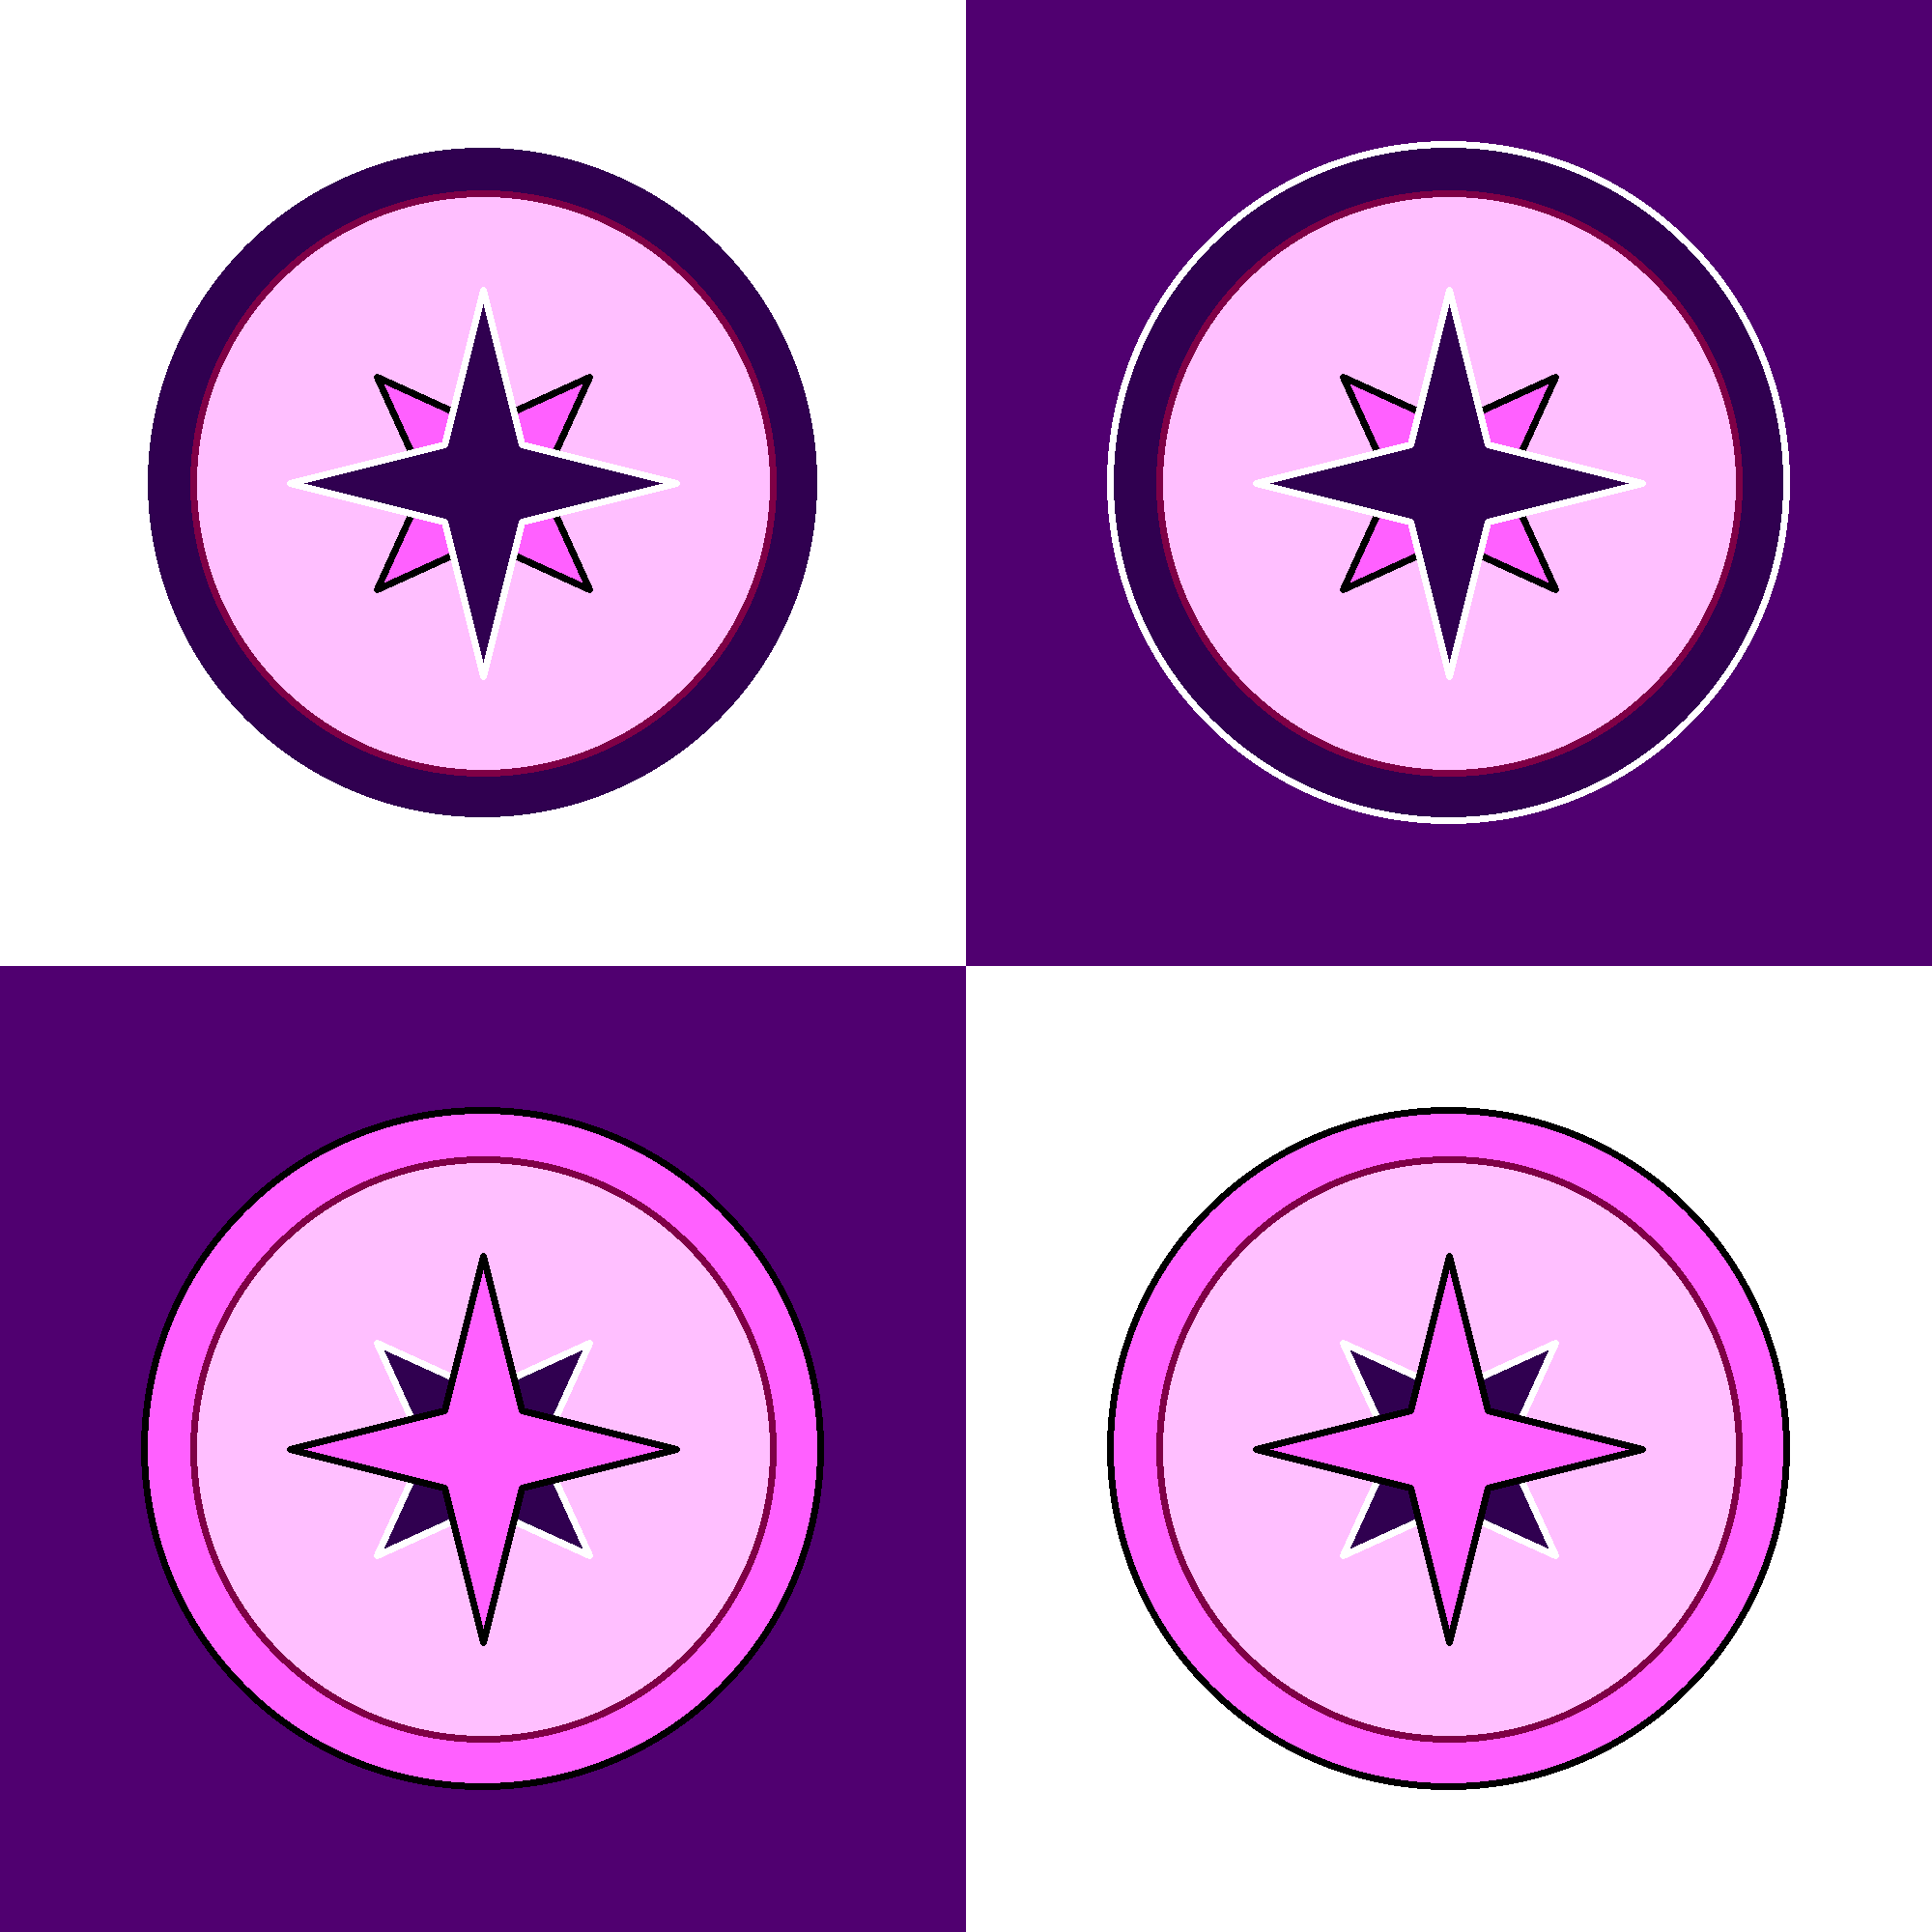
\includegraphics[width=0.4\textwidth, keepaspectratio=true]{pieces/16_starchild.png}
\caption{Starchild}
\label{fig:16_starchild}
\end{wrapfigure}
Starchild is supporting piece, it cannot capture any piece, cannot check or checkmate
opponent's King.

Starchild cannot be converted, but can be activated. If activated, it does not spend
momentum while moving. Starchild can activate any own piece, except King, and can
activate opponent's Starchilds. Starchild can also activate and move Stars, but not
Monoliths.

Starchild can take any piece, except Kings, Stars and Monoliths, for a non-interactive,
viewing-only trance-journey.

% \vspace*{0.15\textheight}
\noindent
\begin{wrapfigure}[10]{l}{0.4\textwidth}
\centering
\includegraphics[width=0.4\textwidth, keepaspectratio=true]{pieces/star/22_one.png}
\caption{Star}
\label{fig:star/22_one}
\end{wrapfigure}
Starchild can't teleport. Starchild moves from starting to empty destination field in
an instant, without ever stepping on any intermediate fields and without interacting
with any pieces on them.

Starchild can ressurect any captured piece.

In algebraic notation, symbol for Starchild is 'I'.

Star colors in this variant are presented above, on the left.

\clearpage % ..........................................................
% Movement ------------------------------------------------------------

\subsection*{Movement}
\addcontentsline{toc}{subsection}{Movement}

\vspace*{-1.1\baselineskip}
\noindent
\begin{figure}[!h]
% \begin{figure}[!t]
\includegraphics[width=1.0\textwidth, keepaspectratio=true]{examples/22_o/scn_o_01_starchild_movement.png}
\caption{Starchild movement}
\label{fig:scn_o_01_starchild_movement}
% \centering
\end{figure}

Starchild can move to any empty field in opposite color to the one it's located on.
Starchild is not hampered by any piece between starting and destination field.

Here, light Starchild in the middle is positioned at dark field, and so can access
any empty light field on chessboard, in a single move.

\clearpage % ..........................................................

\subsubsection*{Neighboring-fields}
\addcontentsline{toc}{subsubsection}{Neighboring-fields}

\vspace*{-0.9\baselineskip}
\noindent
\begin{wrapfigure}[5]{l}{0.4\textwidth}
\centering
\includegraphics[width=0.192307692\textwidth, keepaspectratio=true]{examples/22_o/scn_o_02_neighboring_fields.png}
\caption{Neighboring-fields}
\label{fig:scn_o_02_neighboring_fields}
\end{wrapfigure}
Neighboring-fields are all fields immediately surrounding a piece horizontally, vertically
and diagonally. They are the same as step-fields of a King.

\vspace*{1.1\baselineskip}
\subsubsection*{Activating piece}
\addcontentsline{toc}{subsubsection}{Activating piece}

\vspace*{-0.9\baselineskip}
\noindent
\begin{wrapfigure}[7]{l}{0.4\textwidth}
\centering
\includegraphics[width=0.192307692\textwidth, keepaspectratio=true]{examples/22_o/scn_o_03_starchild_activating_fields.png}
\caption{Activating piece}
\label{fig:scn_o_03_starchild_activating_fields}
\end{wrapfigure}
Fields at which Starchild can activate a piece are neighboring-fields.

Note, Starchild can move only to non-empty activation fields, and only if it contains
own piece, except King, or opponent's Starchids.

Here, Starchild’s activation fields are enumerated. Opponent's Bishop and own King can't
be activated, so only own Pegasus can be, with 1 momentum.

\vspace*{-1.1\baselineskip}
\subsubsection*{Activating Wave}
\addcontentsline{toc}{subsubsection}{Activating Wave}

\vspace*{-0.9\baselineskip}
\noindent
\begin{wrapfigure}[10]{l}{0.4\textwidth}
\centering
\includegraphics[width=0.192307692\textwidth, keepaspectratio=true]{examples/22_o/scn_o_04_starchild_activating_wave_init.png}
\caption{Activating Wave}
\label{fig:scn_o_04_starchild_activating_wave_init}
\end{wrapfigure}
Wave activated by Starchild can activate a piece on its' neighboring-fields, with 1 momentum.
Any own piece, except King, can be activated by Wave, and also opponent's Waves.
Activated Wave can teleport via Star or Monolith, if they are also on Wave's neighboring-fields,
enumerated in this example.

\clearpage % ..........................................................

% \vspace*{-3.1\baselineskip}
\vspace*{-2.1\baselineskip}
\noindent
\begin{figure}[!h]
% \begin{figure}[!t]
\includegraphics[width=1.0\textwidth, keepaspectratio=true]{examples/22_o/scn_o_05_starchild_activating_wave_end.png}
\caption{Teleported Wave}
\label{fig:scn_o_05_starchild_activating_wave_end}
% \centering
\end{figure}

Teleported Wave behaves as described in
\hyperref[fig:scn_n_04_teleport_move_3]{previous variant, Nineteen}.
Here, Wave could e.g. activate light Bishop, or
\hyperref[sec:Terms/Push-pull activation]{push-pull} light Starchild, with 1 momentum.

Other option for activated Wave is to move to any empty field in color opposite to a
color of a starting field. Before teleportation, Wave had all empty, light fields
accessible, because it was initially located on a dark field.

\clearpage % ..........................................................

% \vspace*{-1.1\baselineskip}
\subsubsection*{Moving a Star}
\addcontentsline{toc}{subsubsection}{Moving a Star}

\vspace*{-0.9\baselineskip}
\noindent
\begin{wrapfigure}[5]{l}{0.4\textwidth}
\centering
\includegraphics[width=0.192307692\textwidth, keepaspectratio=true]{examples/22_o/scn_o_06_starchild_moving_star_init.png}
\caption{Moving into a Star}
\label{fig:scn_o_06_starchild_moving_star_init}
\end{wrapfigure}
Starchild's activation fields are enumerated. Starchild can move a Star by activating it,
the same way as any other piece, i.e. by capturing field at which Star is located.

\vspace*{2.1\baselineskip}
\noindent
\begin{wrapfigure}[4]{l}{0.4\textwidth}
\centering
\includegraphics[width=0.192307692\textwidth, keepaspectratio=true]{examples/22_o/scn_o_07_starchild_moving_star_end.png}
\caption{Moving a Star}
\label{fig:scn_o_07_starchild_moving_star_end}
\end{wrapfigure}
Once activated, Star can move to any empty neighboring-field, which all are enumerated in
example on the left.

\clearpage % ..........................................................

% \vspace*{1.1\baselineskip}
\subsubsection*{Not moving a Monolith}
\addcontentsline{toc}{subsubsection}{Not moving a Monolith}

\vspace*{-0.9\baselineskip}
\noindent
\begin{wrapfigure}[5]{l}{0.4\textwidth}
\centering
\includegraphics[width=0.192307692\textwidth, keepaspectratio=true]{examples/22_o/scn_o_08_starchild_not_moving_monolith_init.png}
\caption{Moving into a Monolith}
\label{fig:scn_o_08_starchild_not_moving_monolith_init}
\end{wrapfigure}
Starchild’s activation fields are enumerated. Starchild can try to capture field at which
Monolith is located, as if trying to activate and move it.

\vspace*{2.1\baselineskip}
\noindent
\begin{wrapfigure}[4]{l}{0.4\textwidth}
\centering
\includegraphics[width=0.192307692\textwidth, keepaspectratio=true]{examples/22_o/scn_o_09_starchild_not_moving_monolith_end.png}
\caption{Moving out of a Monolith}
\label{fig:scn_o_09_starchild_not_moving_monolith_end}
\end{wrapfigure}
Instead of moving a Monolith, Starchild then emerges on any empty portal-field around Monolith
it tried to move.

\clearpage % ..........................................................

% \vspace*{1.1\baselineskip}
\subsubsection*{Teleporting Wave}
\addcontentsline{toc}{subsubsection}{Teleporting Wave}

\vspace*{-0.9\baselineskip}
\noindent
\begin{figure}[!h]
% \begin{figure}[!t]
\includegraphics[width=1.0\textwidth, keepaspectratio=true]{examples/22_o/scn_o_10_star_moved_wave_teleportation.png}
\caption{Teleporting Wave}
\label{fig:scn_o_10_star_moved_wave_teleportation}
% \centering
\end{figure}

Stars in this variant can be moved out of their default positions. Teleportation for Wave
reaching a Star is mandatory, step-fields behind a Star are blocked. So, a Star is the only
piece Wave cannot "pass-through", i.e. ignore as all the other pieces on chessboard.

\clearpage % ..........................................................

\vspace*{-2.1\baselineskip}
\noindent
\begin{figure}[!h]
% \begin{figure}[!t]
\includegraphics[width=1.0\textwidth, keepaspectratio=true]{examples/22_o/scn_o_11_star_moved_wave_off_board.png}
\caption{Teleporting Wave}
\label{fig:scn_o_11_star_moved_wave_off_board}
% \centering
\end{figure}

[*] moved Star ---\textgreater Wave \textgreater\textgreater if no board field beyond other Star \textgreater\textgreater sacrified [*]

see \hyperref[fig:scn_d_10_teleported_wave_blocked]{see "Teleported Wave blocked"}

see \hyperref[fig:scn_d_11_wave_teleported_off_board]{see "Wave teleported off-board"}

% ------------------------------------------------------------ Movement
\clearpage % ..........................................................
% Trance-journey ------------------------------------------------------

\subsection*{Trance-journey}
\addcontentsline{toc}{subsection}{Trance-journey}

% \vspace*{-1.3\baselineskip}
\vspace*{-0.9\baselineskip}
\noindent
\begin{wrapfigure}[11]{l}{0.4\textwidth}
\centering
\includegraphics[width=0.346153846\textwidth, keepaspectratio=true]{examples/22_o/scn_o_12_trance_journey_init_starchild.png}
\caption{Starchild initiating}
\label{fig:scn_o_12_trance_journey_init_starchild}
\end{wrapfigure}
Trance-journey is initiated by either Shaman or Starchild, by activating another Starchild.
Activated Starchild then activates a piece, entranced piece then leaves onto trance-journey.
Any piece, own or opponent's, can be entranced, except Kings, Stars and Monoliths.

Between initiating piece and entrancing Starchild only Waves are allowed, but no other pieces.
Initiating Shaman or Starchild can themselves be activated by some other piece(s), not necessarily
in the same color.

% \vspace*{-0.3\baselineskip}
\vspace*{-0.1\baselineskip}
\noindent
\begin{wrapfigure}[10]{l}{0.4\textwidth}
\centering
\includegraphics[width=0.346153846\textwidth, keepaspectratio=true]{examples/22_o/scn_o_13_trance_journey_init_shaman.png}
\caption{Shaman initiating}
\label{fig:scn_o_13_trance_journey_init_shaman}
\end{wrapfigure}
Entranced piece must have the same color as initiating Shaman or Starchild, color of
entrancing Starchild do not need to match.

Here, entranced piece is dark Bishop, both initiating pieces are also dark, i.e. dark Shaman
in this example, and dark Starchild in previous example. Entrancing piece in both examples
is light Starchild.

Entranced piece can end its' trance-journey on any empty step-field. If all are occupied, then it emerges
on any empty entrancing Starchild's neighboring-field. If there's none, then it emerges on empty initiating
Shaman or Starchild's neighboring-fields. If all are occupied, entranced piece is removed from chessboard,
as if captured by opponent.

\clearpage % ..........................................................

\vspace*{-3.1\baselineskip}
\noindent
\begin{figure}[!h]
% \begin{figure}[!t]
\includegraphics[width=1.0\textwidth, keepaspectratio=true]{examples/22_o/scn_o_14_trance_journey_started_by_shaman.png}
\caption{Trance-journey}
\label{fig:scn_o_14_trance_journey_started_by_shaman}
% \centering
\end{figure}

Trance-journey pattern depends on color of entrancing Starchild. Here, light Starchild features
\hyperref[fig:scn_cot_14_light_shaman_trance_journey]{light Shaman's pattern}. Should entrancing
Starchild be dark, it would also produce
\hyperref[fig:scn_cot_16_dark_shaman_trance_journey]{dark Shaman's pattern}.

Trance-journey is optional, entranced piece could just move, with received momentum.
Here, dark Bishop is receiving 1 momentum, so it could move for 1 step.

\clearpage % ..........................................................

% \vspace*{-1.1\baselineskip}
\subsubsection*{Push-pull entrancement}
\addcontentsline{toc}{subsubsection}{Push-pull entrancement}

\vspace*{-0.9\baselineskip}
\noindent
\begin{wrapfigure}[7]{l}{0.4\textwidth}
\centering
\includegraphics[width=0.346153846\textwidth, keepaspectratio=true]{examples/22_o/scn_o_15_push_pull_trance_journey_init.png}
\caption{Initiating trance-journey}
\label{fig:scn_o_15_push_pull_trance_journey_init}
\end{wrapfigure}
Starchild initiating trance-journey could also be activated later in the same cascade, and act as an
entrancing Shaman. This is similar to push-pull entrancement in the
\hyperref[fig:star/scn_cot_33_push_pull_entrancement_start]{previous variant, Conquest of Tlalocan}.

\vspace*{3.9\baselineskip}
% \vspace*{-0.9\baselineskip}
\noindent
\begin{wrapfigure}[10]{l}{0.4\textwidth}
\centering
\includegraphics[width=0.346153846\textwidth, keepaspectratio=true]{examples/22_o/scn_o_16_push_pull_trance_journey_entrancing.png}
\caption{Push-pull entrancing}
\label{fig:scn_o_16_push_pull_trance_journey_entrancing}
\end{wrapfigure}
In previous eample, dark Starchild activated Wave A, which then activated Wave B. Here, Wave B is
"in the air", about to activate dark Starchild, which will then entrance dark Knight.

\clearpage % ..........................................................

% \vspace*{-3.1\baselineskip}
\noindent
\begin{figure}[!h]
% \begin{figure}[!t]
\includegraphics[width=1.0\textwidth, keepaspectratio=true]{examples/22_o/scn_o_17_push_pull_trance_journey_entranced.png}
\caption{Dark-pattern trance-journey}
\label{fig:scn_o_17_push_pull_trance_journey_entranced}
% \centering
\end{figure}

Starchild can initiate trance-journey by
\hyperref[sec:Terms/Push-pull activation]{push-pull activation},
if its' color is the same as color of entranced piece; here both Starchild and Knight are dark.

Push-pull activation would work even if initiating Starchild has been activated by some other pieces,
which don't have to be in the same color.

% ------------------------------------------------------ Trance-journey
\clearpage % ..........................................................

\subsection*{Syzygy}
\addcontentsline{toc}{subsection}{Syzygy}

[*] Syzygy (+?) ... --\textgreater ressurection [*]

% *********************************************************** Starchild
\clearpage % ..........................................................

\section*{Promotion}
\addcontentsline{toc}{section}{Promotion}

Promotion is non enforced, delayed variety, i.e. it's the same as in
\hyperref[sec:Age of Aquarius/Promotion]{previous chess variant}, Age of Aquarius.

Additionaly, promotion in this variant is monogamous.
Only one Queen in the same color can be present on chessboard at any given time.

\clearpage % ..........................................................

\section*{Rush, en passant}
\addcontentsline{toc}{section}{Rush, en passant}

\vspace*{-1.2\baselineskip}
\noindent
\begin{figure}[!h]
% \begin{figure}[!t]

\includegraphics[width=1.0\textwidth, keepaspectratio=true]{en_passants/22_one_en_passant.png}
\caption{En passant}
\label{fig:22_one_en_passant}
% \centering
\end{figure}

Rush and en passant are identical to those in \hyperref[fig:14_hemera_s_dawn_en_passant]{Hemera's Dawn variant}.
Own Pawns can be rushed for up to 11 fields in this variant.

\clearpage % ..........................................................

\section*{Castling}
\addcontentsline{toc}{section}{Castling}

Castling is the same as in Classical Chess, only difference is that King can move between 2 and 10 fields across.
All other constraints from Classical Chess still applies.

\noindent
\begin{figure}[!h]
% \begin{figure}[!t]
\includegraphics[width=1.0\textwidth, keepaspectratio=true]{castlings/22_o/one_castling.png}
\caption{Castling}
\label{fig:one_castling}
% \centering
\end{figure}

In example above, all valid King's castling moves are numbered.

\noindent
\begin{figure}[!h]
% \begin{figure}[!t]
\includegraphics[width=1.0\textwidth, keepaspectratio=true]{castlings/22_o/one_castling_right_04.png}
\caption{Castling short right}
\label{fig:one_castling_right_04}
% \centering
\end{figure}

In this example King was castling short to the right. Initial King's position is marked with "K".
After castling is finished, right Rook ends up at field immediately left to the King.

\clearpage % ..........................................................

\section*{Initial setup}
\addcontentsline{toc}{section}{Initial setup}

Compared to initial setup of Discovery, Starchild is inserted between Unicorn and Shaman
symmetrically, on both sides of chessboard. This can be seen in the image below:

\noindent
% \begin{figure}[t]
\begin{figure}[h]
\includegraphics[width=1.0\textwidth, keepaspectratio=true]{boards/22_one.png}
\caption{One board}
\label{fig:22_one}
% \centering
\end{figure}

\clearpage % ..........................................................
% ========================================================= One chapter
